%!TEX root = ../dissertation.tex

\chapter{Evaluation}
\label{chapter:results}

This chapter describes the methods used for benchmarking the proposed case study
and their respective results.
The first part describes the real world benchmark setup, robot and domestic environment, whereas
on the second part, it is described the simulation benchmark, based on synthetic sensor data from
possible scenarios in the domestic environment. This includes an observation set given to the program 
on each benchmark test and the results for that same test.

\subsection{Physical Setup}

\subsubsection{Robot Platform}
An omni-directional 4-wheeled robot with a torso and rotating head. It is configured with 
two laser range finders (front and back of its base), Kinect 1 camera on the front of the head, 
plus an additional Asus Xtion PRO Live camera
and a directional microphone R{\o}de VideoMic Pro on top of its head for speech recognition. It also
includes a robotic manipulator Robai Cyton Gamma 1500 which was not used due to hardware and software 
problems at the time.

\begin{figure}[H]
    \centering
        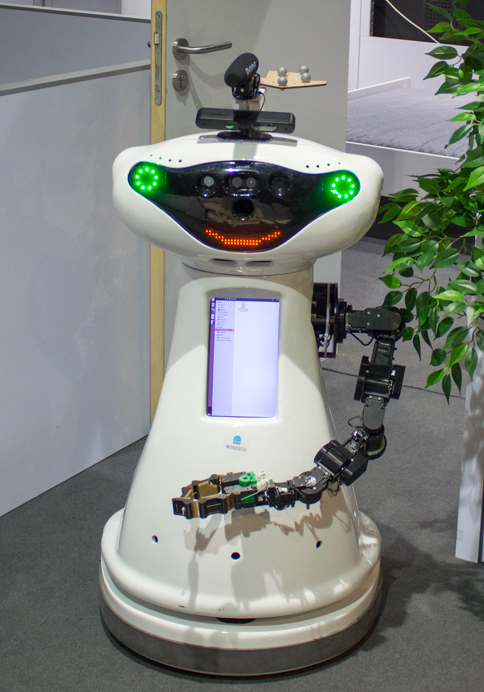
\includegraphics[scale=0.3]{images/mbot}
        \caption{\textit{Mbot}, the robot that was used for the real world benchmarks.}
        \label{fig:mbot}
\end{figure}

\subsubsection{ISRoboNet@Home - Home Environment Testbed}
Located in Instituto de Sistemas e Robótica, Lisbon. 
Serves as a benchmarking tool for robot's performance while on domestic environments. 
In figure \ref{fig:testbed}, it includes a kitchen, bedroom, dining and living room, all
fully furnished with commonly found appliances from \textit{IKEA} store. This
makes it easy to recreate similar environments on different laboratories and
competitions across the world or in simulation environments, like \textit{Gazebo}.

\begin{figure}[H]
    \centering
        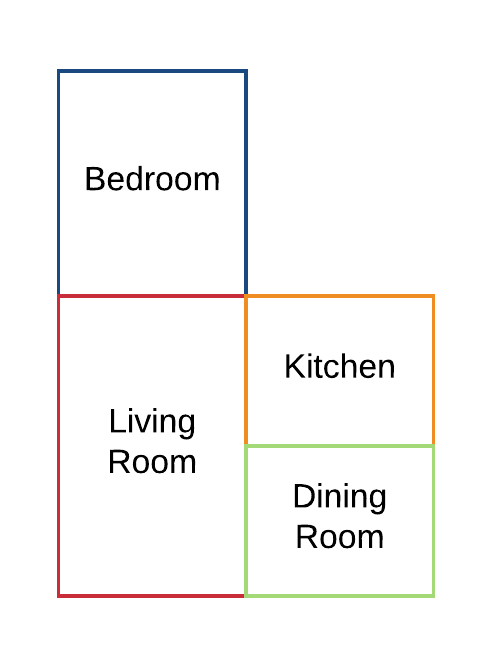
\includegraphics[scale=1]{images/testbed_map}
        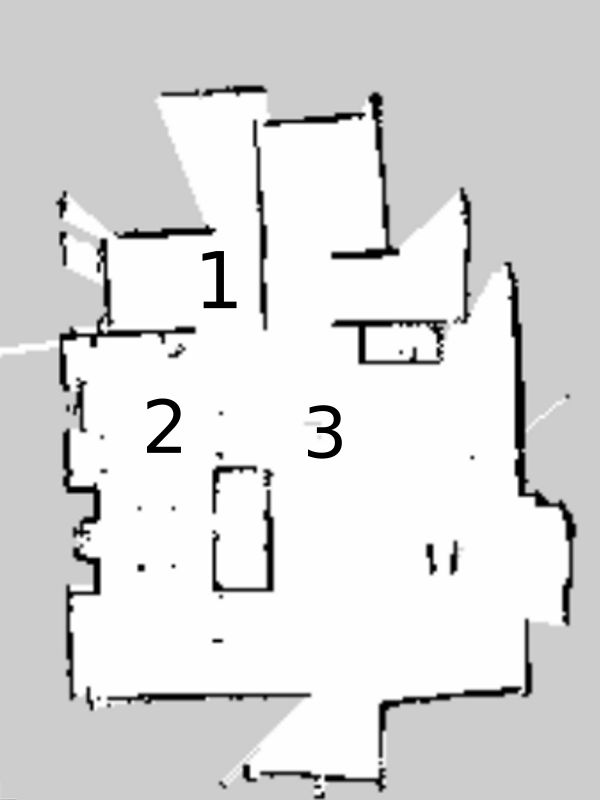
\includegraphics[scale=0.25]{images/home_map}
        \caption{On the left image, it can be seen a topological map of the
        ISRoboNet@Home testbed. On the right image, it is shown the map used
        by the robot for navigation and localization.}
        \label{fig:testbed}
\end{figure}

\section{Simulation Benchmark Setup}

First and foremost, all tests were performed on a single machine, equipped with
an Intel i7 4700MQ CPU, 8 GB of RAM, on Ubuntu 16.04 KDE as operating system.
The tests were performed on isolated environments with docker containers, so
that they could be easily reproduced with minimum work on other computers or
robotic platforms. The computer ran the tests while having the minimum amount of
resources needed to
operate. This means the computer was left alone to run these tests.
Every benchmark test was executed 5 times to have a better estimate of its
expected action choice, action-value estimates and its variance. Similarly, it
was measured the time it took to return some output, with the same statistical
estimators as before. It is also important to mention that a minimal number of
tests were interrupted by the prolog's engine core dumps and so, their execution
was ignored.

The description of the task consists of three parts:
\begin{itemize}
	\item On the first part, the robot is idle in the sofa location. Suddenly, he 
    is called by Robert. So, he should move to Robert's location (which is the bed).
    Afterwards, he should engage in conversation with Robert, in order to confirm the
    initial call and ask what he needs. At this point, Robert requests a coke beverage 
    and the robot should acknowledge this request.
    \item The second part relates to the mission domain where the robot needs to deliver
    the coke to Robert. He will have two choices: ask for help to get the coke; or grasp it
    and deliver it himself. But, in this case, the coke is already in the same location as 
    Robert and the robot and, the latter is near it. So, the expected result should be the
    robot grasping and delivering the object himself, without any assistance.
    \item The third part is similar to the previous one, but now the coke is in the kitchen table
    instead of the bed. So, the robot should move to the kitchen table location and request assistance
    to Lynda so that he can return to bed location and deliver the object to Robert.
\end{itemize}

\subsection{Results}

The following results were obtained with 300 episodes/samples and a maximum of 
10 steps on a running episode with $\gamma=0.9$. The three following tables 
\ref{tab:results_one}, \ref{tab:results_two} and \ref{tab:results_three} 
represent each test referred before.

\begin{table}[H]
\centering
\begin{tabular}{ |c|c|c|c| }
 \hline
Step \# & Best Action                                          &  Time (s) \\
 \hline
1       & wait                                                 & 180               \\
2       & navigate(bed)                                        & 219               \\
3       & respond(ready\_to\_help, robert)                     & 202               \\
4       & respond(robert, confirm\_mission, want(robert,coke)) & 147              \\
\hline
\end{tabular}
\label{tab:results_one}
\caption{First case study results on the Wandering Domain.}
\end{table}


\begin{table}[H]
\centering
\begin{tabular}{ |c|c|c|c| }
 \hline
Step \# & Best Action                                          &  Time (s) \\
 \hline
1       & grasp(coke)                                          & 263               \\
2       & deliver(coke, robert)                                & 109               \\
\hline
\end{tabular}
\label{tab:results_two}
\caption{Second case study results on the Mission Domain.}
\end{table}

\begin{table}[H]
\centering
\begin{tabular}{ |c|c|c|c| }
 \hline
Step \# & Best Action                                          &  Time (s) \\
 \hline
1       & navigate(kitchen\_table)                              & 326               \\
2       & ask\_help(coke, lynda)                                & 292               \\
3       & navigate(bed)                                         & 264               \\
4       & receive(coke, lynda)                                  & 182               \\
5       & deliver(coke, robert)                                 & 105               \\
\hline
\end{tabular}
\label{tab:results_three}
\caption{Third case study results on the Mission Domain.}
\end{table}

\section{Experimental Procedure}

The experimental case studies were executed with help from people that were present
in the lab at the time (test subjects). Then, test subjects would show QR codes to 
the robot which represented the external sensor information the robot would receive in 
a real scenario (as shown in figure \ref{fig:real_world_test_wander}). These physical 
experiments are just a proof of concept of the planned design, since sensor information was prefabricated.
Tests were made to replicate the behavior which was obtained on simulation scenario.
Video demonstration of the experiments can be seen in \url{www.youtube.com}.

\begin{figure}[H]
    \centering
        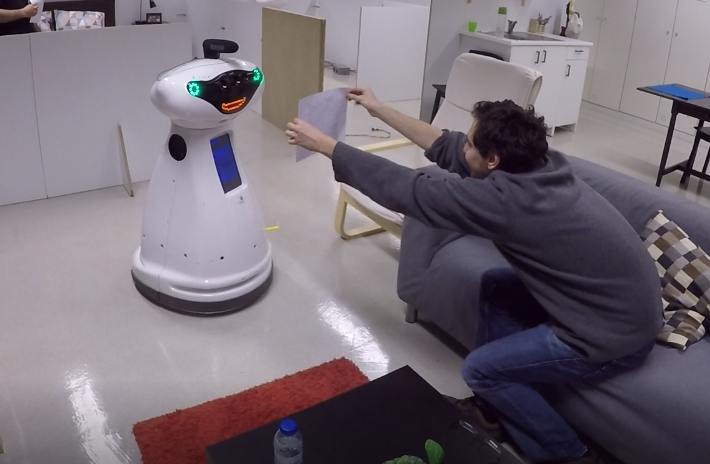
\includegraphics[scale=0.3]{images/realtest1}
        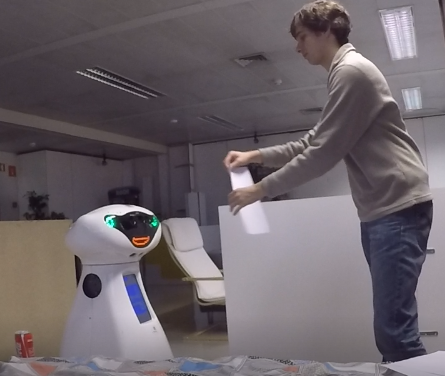
\includegraphics[scale=0.37]{images/realtest3}
        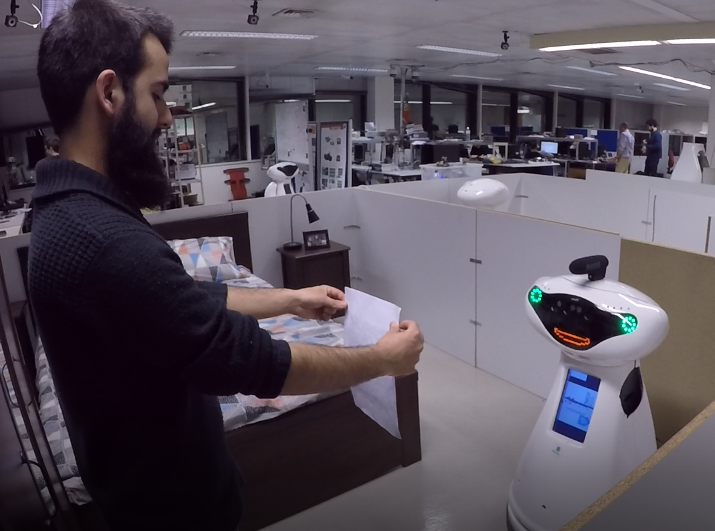
\includegraphics[scale=0.27]{images/realtest2}
        \caption{Robot in a real world benchmark, on the mission domain
        situation, with a real human giving external sensor information with a
        QR code. On the left, the robot is in the initial sofa location; on the center
        the robot is simulating a coke grasp; on the right, the robot is in the bed location,
        also next to robert and trying to deliver the object to him.}
        \label{fig:real_world_test_wander}
\end{figure}
